\documentclass[tikz,border=6pt]{standalone}
\usepackage{amsmath}
\usepackage{amssymb}
\usetikzlibrary{arrows.meta,calc,positioning}

\begin{document}

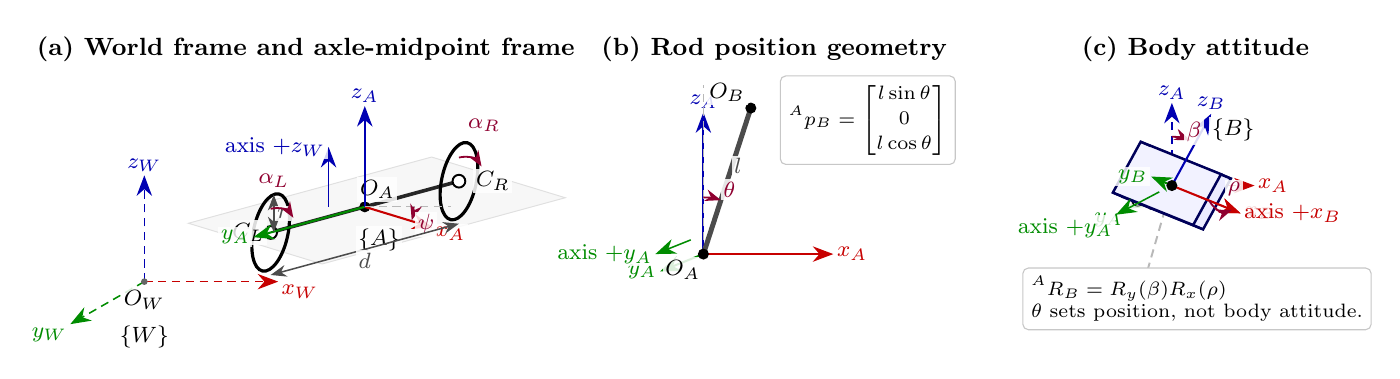
\begin{tikzpicture}[
  >=Stealth,
  xaxis/.style={red!78!black, -{Stealth[length=2.6mm]}, line width=0.75pt},
  yaxis/.style={green!55!black, -{Stealth[length=2.6mm]}, line width=0.75pt},
  zaxis/.style={blue!70!black, -{Stealth[length=2.6mm]}, line width=0.75pt},
  refaxis/.style={dash pattern=on 3pt off 2pt, line width=0.55pt},
  body/.style={draw=blue!35!black, fill=blue!8, line width=0.9pt},
  bodyedge/.style={draw=blue!35!black, line width=0.8pt},
  structure/.style={black!85, line width=1.3pt},
  rod/.style={black!70, line width=1.8pt},
  guide/.style={black!28, dash pattern=on 3pt off 2pt, line width=0.45pt},
  dimension/.style={black!70, {Stealth[length=2.0mm]}-{Stealth[length=2.0mm]}, line width=0.55pt},
  angle/.style={purple!75!black, -{Stealth[length=2.0mm]}, line width=0.65pt},
  axislabel/.style={font=\footnotesize, inner sep=1pt, fill=white, fill opacity=0.82, text opacity=1},
  smalllabel/.style={font=\footnotesize, inner sep=1pt, fill=white, fill opacity=0.86, text opacity=1},
  titlelabel/.style={font=\bfseries\small},
  formula/.style={font=\scriptsize, align=left, fill=white, draw=black!22, rounded corners=2pt, inner sep=3pt}
]

% --------------------------------------------------------------------------
% Global drawing convention:
% The figure is a 2.5D engineering schematic.  Panel (a) uses a fixed oblique
% projection for the horizontal plane: X -> (1,0), Y -> (-0.55,-0.32),
% Z -> (0,1).  Panels (b) and (c) use simplified projected views chosen for
% clarity, not perspective rendering.
% --------------------------------------------------------------------------

\def\psia{32}     % displayed yaw angle
\def\thetaa{18}   % displayed leg angle
\def\betaa{22}    % displayed body pitch
\def\rhoa{22}     % displayed body roll

\colorlet{xcol}{red!78!black}
\colorlet{ycol}{green!55!black}
\colorlet{zcol}{blue!70!black}
\colorlet{angcol}{purple!75!black}

% ==========================================================================
% (a) World frame and axle-midpoint frame
% ==========================================================================
\begin{scope}[shift={(0,0)}]
  \node[titlelabel] at (2.25,3.05) {(a) World frame and axle-midpoint frame};

  % Fixed oblique basis in the horizontal plane.
  \coordinate (OW) at (0.20,0.10);
  \coordinate (xWend) at ($(OW)+(1.70,0)$);
  \coordinate (yWend) at ($(OW)+(-0.94,-0.54)$);
  \coordinate (zWend) at ($(OW)+(0,1.35)$);

  % Current axle midpoint O_A and A axes.  Derived from yaw in the projected
  % horizontal plane: x_A = cos(psi) X_W + sin(psi) Y_W,
  % y_A = -sin(psi) X_W + cos(psi) Y_W.
  \pgfmathsetmacro{\xAx}{cos(\psia) - 0.55*sin(\psia)}
  \pgfmathsetmacro{\xAy}{-0.32*sin(\psia)}
  \pgfmathsetmacro{\yAx}{-sin(\psia) - 0.55*cos(\psia)}
  \pgfmathsetmacro{\yAy}{-0.32*cos(\psia)}
  \coordinate (OA) at (3.00,1.05);
  \coordinate (xAend) at ($(OA)+1.55*(\xAx,\xAy)$);
  \coordinate (yAend) at ($(OA)+1.42*(\yAx,\yAy)$);
  \coordinate (zAend) at ($(OA)+(0,1.28)$);

  % Symmetric wheel centers along +/- y_A.
  \coordinate (CL) at ($(OA)+1.20*(\yAx,\yAy)$);
  \coordinate (CR) at ($(OA)-1.20*(\yAx,\yAy)$);

  % Pale ground plane.
  \filldraw[fill=black!3, draw=black!12, line width=0.35pt]
    ($(OA)-1.25*(\xAx,\xAy)-1.55*(\yAx,\yAy)$) --
    ($(OA)+1.80*(\xAx,\xAy)-1.55*(\yAx,\yAy)$) --
    ($(OA)+1.80*(\xAx,\xAy)+1.55*(\yAx,\yAy)$) --
    ($(OA)-1.25*(\xAx,\xAy)+1.55*(\yAx,\yAy)$) -- cycle;

  % World frame.
  \draw[xaxis, refaxis] (OW) -- (xWend) node[axislabel, below right] {$x_W$};
  \draw[yaxis, refaxis] (OW) -- (yWend) node[axislabel, below left] {$y_W$};
  \draw[zaxis, refaxis] (OW) -- (zWend) node[axislabel, above] {$z_W$};
  \fill[black!60] (OW) circle (1.2pt);
  \node[smalllabel, below=2pt of OW] {$O_W$};
  \node[smalllabel] at ($(OW)+(0,-0.70)$) {$\{W\}$};

  % Axle and wheels.
  \draw[structure] (CL) -- (CR);
  \draw[black, line width=1.15pt] (CL) ellipse [x radius=0.22, y radius=0.50, rotate=-12];
  \draw[black, line width=1.15pt] (CR) ellipse [x radius=0.22, y radius=0.50, rotate=-12];
  \fill[white, draw=black, line width=0.7pt] (CL) circle (2.3pt);
  \fill[white, draw=black, line width=0.7pt] (CR) circle (2.3pt);
  \fill[black] (OA) circle (2.0pt);
  \node[smalllabel, left=1pt of CL] {$C_L$};
  \node[smalllabel, right=5pt of CR] {$C_R$};
  \node[smalllabel] at ($(OA)+(0.16,0.22)$) {$O_A$};

  % A frame.
  \draw[xaxis] (OA) -- (xAend);
  \node[axislabel, text=xcol] at ($(xAend)+(0.22,-0.08)$) {$x_A$};
  \draw[yaxis] (OA) -- (yAend) node[axislabel, left] {$y_A$};
  \draw[zaxis] (OA) -- (zAend) node[axislabel, above] {$z_A$};
  \node[smalllabel] at ($(OA)+(0.18,-0.42)$) {$\{A\}$};

  % Yaw angle in ground plane, from x_W to x_A.  Axis is z_W/z_A.
  \draw[guide] (OA) -- ($(OA)+(1.10,0)$);
  \draw[angle] ($(OA)+(0.62,0)$) arc[start angle=0, end angle=-16, radius=0.62];
  \node[smalllabel, text=angcol] at ($(OA)+(0.78,-0.22)$) {$\psi$};
  \draw[zaxis, line width=0.55pt] ($(OA)+(-0.46,0.00)$) -- ++(0,0.76)
    node[axislabel, left] {axis $+z_W$};

  % Track dimension d.
  \draw[dimension] ($(CL)+(0,-0.54)$) -- ($(CR)+(0,-0.54)$)
    node[midway, below, smalllabel] {$d$};

  % Wheel radius r on left wheel.
  \draw[dimension] ($(CL)+(0.04,0)$) -- ++(0,0.48)
    node[midway, right, smalllabel] {$r$};

  % Wheel rotation angles.
  \draw[angle] ($(CL)+(0.00,0.30)$) arc[start angle=105, end angle=32, radius=0.26];
  \node[smalllabel, text=angcol] at ($(CL)+(0.04,0.66)$) {$\alpha_L$};
  \draw[angle] ($(CR)+(0.00,0.30)$) arc[start angle=105, end angle=32, radius=0.26];
  \node[smalllabel, text=angcol] at ($(CR)+(0.32,0.71)$) {$\alpha_R$};
\end{scope}

% ==========================================================================
% (b) Rod position geometry in the x_A-z_A side view
% ==========================================================================
\begin{scope}[shift={(6.25,0)}]
  \node[titlelabel] at (1.95,3.05) {(b) Rod position geometry};

  \coordinate (OA2) at (1.05,0.45);
  \pgfmathsetmacro{\legx}{1.95*sin(\thetaa)}
  \pgfmathsetmacro{\legz}{1.95*cos(\thetaa)}
  \coordinate (OB2) at ($(OA2)+(\legx,\legz)$);

  % Reference frame A in side view.
  \draw[xaxis] (OA2) -- ++(1.65,0) node[axislabel, right] {$x_A$};
  \draw[zaxis] (OA2) -- ++(0,1.80) node[axislabel, above] {$z_A$};
  \draw[yaxis] (OA2) -- ++(-0.55,-0.22) node[axislabel, left] {$y_A$};
  \node[smalllabel, below left=1pt and 0pt of OA2] {$O_A$};

  % Auxiliary vertical ray and true rod.
  \draw[guide] (OA2) -- ++(0,2.15);
  \draw[rod] (OA2) -- (OB2) node[midway, above right=1pt, smalllabel] {$l$};
  \fill[black] (OA2) circle (2.0pt);
  \fill[black] (OB2) circle (2.0pt);
  \node[smalllabel, above left=1pt and 1pt of OB2] {$O_B$};

  % theta: from +z_A to rod direction, centered at O_A, axis +y_A.
  \draw[angle] ($(OA2)+(0,0.72)$) arc[start angle=90, end angle={90-\thetaa}, radius=0.72];
  \node[smalllabel, text=angcol] at ($(OA2)+(0.33,0.82)$) {$\theta$};
  \draw[yaxis, line width=0.55pt] ($(OA2)+(-0.16,0.18)$) -- ++(-0.45,-0.18)
    node[axislabel, left] {axis $+y_A$};

  % Position formula.
  \node[formula, anchor=north west] at (2.02,2.72)
    {$\displaystyle {}^A p_B=
      \begin{bmatrix}
        l\sin\theta\\[1pt]0\\[1pt]l\cos\theta
      \end{bmatrix}$};
\end{scope}

% ==========================================================================
% (c) Body attitude: pitch beta and roll rho
% ==========================================================================
\begin{scope}[shift={(11.30,0)}]
  \node[titlelabel] at (2.25,3.05) {(c) Body attitude};

  \coordinate (OB3) at (1.95,1.32);

  % Projected reference A basis for this panel.
  \coordinate (xA3) at (1.00,0.00);
  \coordinate (yA3) at (-0.46,-0.24);
  \coordinate (zA3) at (0.00,1.00);

  % Pitch around +y_A:
  % z_P = sin(beta) x_A + cos(beta) z_A,
  % x_P = cos(beta) x_A - sin(beta) z_A.
  \pgfmathsetmacro{\xPx}{cos(\betaa)}
  \pgfmathsetmacro{\xPz}{-sin(\betaa)}
  \pgfmathsetmacro{\zPx}{sin(\betaa)}
  \pgfmathsetmacro{\zPz}{cos(\betaa)}

  % Roll around local x_P:
  % y_B = cos(rho)y_A + sin(rho)z_P,
  % z_B = -sin(rho)y_A + cos(rho)z_P.
  \pgfmathsetmacro{\yBx}{cos(\rhoa)*(-0.46) + sin(\rhoa)*\zPx}
  \pgfmathsetmacro{\yBz}{cos(\rhoa)*(-0.24) + sin(\rhoa)*\zPz}
  \pgfmathsetmacro{\zBx}{-sin(\rhoa)*(-0.46) + cos(\rhoa)*\zPx}
  \pgfmathsetmacro{\zBz}{-sin(\rhoa)*(-0.24) + cos(\rhoa)*\zPz}

  % Faint rod context, without theta/l labels.
  \draw[guide, line width=0.7pt] ($(OB3)+(-0.36,-1.25)$) -- (OB3);

  % A reference directions.
  \draw[xaxis, refaxis] (OB3) -- ++(1.05,0) node[axislabel, right] {$x_A$};
  \draw[yaxis, refaxis] (OB3) -- ++(-0.58,-0.30) node[axislabel, below left] {$y_A$};
  \draw[zaxis, refaxis] (OB3) -- ++(0,1.05) node[axislabel, above] {$z_A$};
  \node[smalllabel, below left=1pt and 1pt of OB3] {$O_B$};

  % Body cuboid as a projected parallelogram with depth.
  \coordinate (B1) at ($(OB3)-0.55*(\xPx,\xPz)-0.34*(\zBx,\zBz)-0.22*(\yBx,\yBz)$);
  \coordinate (B2) at ($(OB3)+0.55*(\xPx,\xPz)-0.34*(\zBx,\zBz)-0.22*(\yBx,\yBz)$);
  \coordinate (B3) at ($(OB3)+0.55*(\xPx,\xPz)+0.34*(\zBx,\zBz)-0.22*(\yBx,\yBz)$);
  \coordinate (B4) at ($(OB3)-0.55*(\xPx,\xPz)+0.34*(\zBx,\zBz)-0.22*(\yBx,\yBz)$);
  \coordinate (B5) at ($(B1)+0.44*(\yBx,\yBz)$);
  \coordinate (B6) at ($(B2)+0.44*(\yBx,\yBz)$);
  \coordinate (B7) at ($(B3)+0.44*(\yBx,\yBz)$);
  \coordinate (B8) at ($(B4)+0.44*(\yBx,\yBz)$);
  \filldraw[body] (B1)--(B2)--(B3)--(B4)--cycle;
  \filldraw[body, fill=blue!5] (B5)--(B6)--(B7)--(B8)--cycle;
  \draw[bodyedge] (B1)--(B5) (B2)--(B6) (B3)--(B7) (B4)--(B8);

  % B frame, solid.
  \draw[xaxis] (OB3) -- ++(0.94*\xPx,0.94*\xPz) node[axislabel, right] {$x_B$};
  \draw[yaxis] (OB3) -- ++(0.92*\yBx,0.92*\yBz) node[axislabel, left] {$y_B$};
  \draw[zaxis] (OB3) -- ++(0.96*\zBx,0.96*\zBz) node[axislabel, above] {$z_B$};
  \fill[black] (OB3) circle (2.0pt);
  \node[smalllabel] at ($(OB3)+(0.78,0.70)$) {$\{B\}$};

  % beta: rotation about +y_A from z_A to pitched z_P.
  \draw[yaxis, line width=0.55pt] ($(OB3)+(-0.16,-0.08)$) -- ++(-0.55,-0.29)
    node[axislabel, below left] {axis $+y_A$};
  \draw[angle] ($(OB3)+(0,0.62)$) arc[start angle=90, end angle={90-\betaa}, radius=0.62];
  \node[smalllabel, text=angcol] at ($(OB3)+(0.28,0.68)$) {$\beta$};

  % rho: subsequent local roll about x_B.  Draw near the x_B axis, with
  % local x axis explicitly indicated.
  \coordinate (rollCenter) at ($(OB3)+0.58*(\xPx,\xPz)$);
  \draw[xaxis, line width=0.55pt] ($(rollCenter)-0.22*(\xPx,\xPz)$) --
    ($(rollCenter)+0.36*(\xPx,\xPz)$) node[axislabel, right] {axis $+x_B$};
  \draw[angle] ($(rollCenter)+0.22*(\yBx,\yBz)$)
    arc[start angle=205, end angle=290, radius=0.23];
  \node[smalllabel, text=angcol] at ($(rollCenter)+(0.25,0.17)$) {$\rho$};

  \node[formula, anchor=north west] at (0.05,0.28)
    {$\displaystyle {}^A R_B=R_y(\beta)R_x(\rho)$\\
     $\theta$ sets position, not body attitude.};
\end{scope}

\end{tikzpicture}

\end{document}
